\section{The Discovery of the Higgs Boson \cite{higgs}}
The discovery of the Higgs boson was finally announced on the 4th of July 2012. The ATLAS and CMS collaborations both confirmed the discovery of a Higgs like particle. The discovery of the Higgs boson closed some serious questions of the Standard Model like the origin of mass.
\subsection{Theoretical principle}
The Standard Model describes the properties and interactions of elementary particles with gauge theories. It was experimemtally determined, that several particles carry a mass. The problem is that the electroweak symmetry requires massless particles, since the explicit mass terms would break it. A possible solution was proposed in 1964: the Higgs mechanism. The Higgs field $\Phi$ is a isospin doublet of complex scalar fields:
\begin{align*}
  \Phi &=
	\begin{pmatrix}
		\Phi^+ \\
		\Phi^0
		\end{pmatrix}
	= \frac{1}{\sqrt{2}}
  \begin{pmatrix}
    \Phi_1 + i \Phi_2 \\
    \Phi_3 + i \Phi_4
  \end{pmatrix}
		& <\Phi> = \frac{1}{\sqrt{2}}
		\begin{pmatrix}
			0 \\
			v
		\end{pmatrix}
		& \;\; \text{with} \;\; v = \sqrt{-\frac{\mu^2}{\lambda}}
\end{align*}
The Higgs potential has the shape of a \textit{mexican hat} and therefore the electroweak symmetry is spontaneously broken. The initial Higgs field has four degrees of freedom. After the spontaneous symmetry breaking (SSB) three are observed by the weak gauge boson masses and the forth leads to the Higgs Boson. The development around the minimum leads to explicit mass terms for the gauge bosons $W^{\pm}$ and $Z^0$. In addition, the fermions get their masses by the Yukawa interaction and couple to the Higgs Boson. \\
The Higgs boson is a scalar particle with Spin 0. It couples to all particles proportional to their mass and due to the selfcoupling term gets a mass itself. Due to the high mass it has a short lifetime. The Higgs boson can be produced via fusion or radiation of massive particles since it couples to mass. The most likely production of the Higgs boson is due to gluon fusion, that couples to a quark loop or decays into a $q\bar{q}$ pair. But even under the LHC conditions the probability for Higgs production is extremely small. There is just one in $10^9$ events. In principle the Higgs boson can decay in every massive particle, but the upper limit is $m_H\approx \frac{m_{decay}^2}{2}$. Decays into $Z\gamma$ or $gg$ are also possible via loops. The problem for predictions was, that the branching fraction highly depends on the actual mass of the Higgs boson and many channels have a high background.
\subsection{Statistics}
The Higgs boson creates a signal excess at a specific invariant mass. Due to the high backgrounds that can also fluctuate, it is important to evaluate the significance of the signal carefully. Different terms of the statistics are important to understand in order to understand why the discovery of the Higgs boson was possible.\\
The signal strength $\mu$ is directly connected to the counting rate $n=\mu(\text{signal})+\text{background}$ and defined by $\mu = \frac{\sigma(m_H)}{\sigma_{\text{SM}}(m_H)}$. \textcolor{red}{A hypothesis gives the probability of a set of possible results}. The \textit{p-value} gives the probability for the excess to be generated by a fluctuation under the hypothesis that there is no signal. The smaller the the p-value is the less likely is the hypothesis. The \textit{level of significance} is a chosen level $\alpha$ to reject the hypothesis for $p<\alpha$. The \textit{confidence interval} contains the true values with a specific probability. In particle physics the usually chosen \textit{confidence level} (CL) is \SI{95}{\percent} CL. This allows to set limits based on measured data with a specific CL.
The Likelihood ratio $q_0 = -2 \log \left(\frac{L(BG)}{L(\mu S+BG)}\right)$ can be used to reject a hypothesis if $q_0>\alpha$, but it is not reliable for low sensitivity experiments since the distributions are too similar.\\
For the $CL_s$ method two pdfs of the test statistic $Q$ are created with a fixed mass hypothesis. One distribution is created with the background and one with the background with signal hypothesis. Afterwards the $p$ value of both distributions is calculated respectivley to the observed $Q_{/text{obs}}$. The \textit{signal confidence value} is thus $CL_s = \frac{p(S+BG)}{1-p(BG)}$. The signal-background hypothesis is rejected at \SI{95}{\percent} CL for $CL_s\leq 0.05$.
\subsection{Previous results}
The CDF and D\O\; collaborations at Tevatron set the Higgs mass limits to be either $m_H<\SI{162}{\GeV}$ or $m_H>\SI{166}{\GeV}$ at \SI{95}{\percent} CL. The experiments at the LEP collider performed $\chi^2$ tests to precision measurements of electroweak observables. This allows to extract limits for the mass $m_H$ of the Higgs boson, since the Higgs boson contributes to loop corrections to the electroweak propagator. The best fit value was between $95$ and \SI{105}{\GeV}, but this region was already excluded by direct searches. Together with other results from direct searches the limit was set to $m_H < \SI{158}{\GeV}$.

\subsection{The Discovery at the LHC}
\begin{wrapfigure}{l}{0.4\textwidth}
    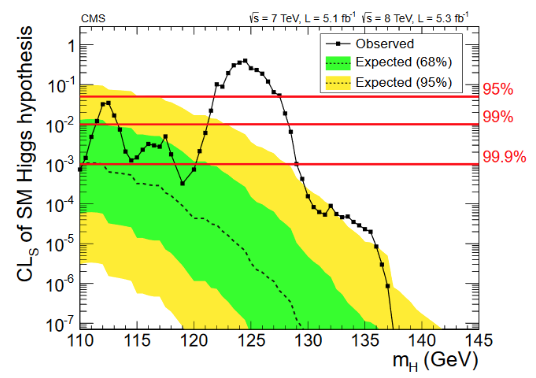
\includegraphics[width=0.38\textwidth]{graphics/higgs.png}
    \caption{$CL_s$ test for the Higgs boson mass hypothesis of $m_h\approx\SI{125}{\GeV}$. \cite{higgs}}
  \end{wrapfigure}
  \FloatBarrier
The LHC is a \SI{27}{\kilo\meter} hadron collider build to discover the Higgs boson. The LHC contains two general purpose detectors, ATLAS and CMS, with the main goal to find the Higgs boson. Their physics programme also contains the search for new physics e.g. SUSY particles. The idea was to build two experiments to independently validate the results and minimize systematic uncertainties with different detector designs. Both experiments contain a tracking system, a solenoid, calorimeters and muon detectors. The main difference is that ATLAS placed the solenoid before the calorimeters, while CMS placed the solenoid behind them.\\
ATLAS and CMS mainly concentrated on the two channels $H\rightarrow ZZ^* \rightarrow 4l$ and $H\rightarrow \gamma\gamma$ since they have the best properties for discovery. Other channels have a significantly larger background due to undetectable neutrinos or QCD processes that produce further jets.\\
Both collaborations could exclude masses above \SI{129}{\GeV}, but had no signifcant excess around \SI{125}{\GeV} with the data from the 2011 run. The LHC increased the center of mass energy in 2012 from \SI{7}{\TeV} to \SI{8}{\TeV}. This led to a higher luminosity and increased the production cross section. Both collaborations performed $CL_s$ tests at a \SI{95}{\percent} CL. ATLAS could not exclude $122<m_H<\SI{131}{\GeV}$ and CMS $122<m_H<\SI{131}{\GeV}$ at the \SI{95}{\percent} CL. Together with the 2011 and 2012 data sets they finally reached significant excesses and published the dicovery of a Higgs like particle with 5.9(ATLAS) and 5.0 (CMS) standard deviations in june 2012. The new scalar had a mass of
\begin{align*}
	m_H &= 126.0 \pm 0.4\pm0.4 \;\si{\GeV} \;\;(\text{ATLAS})\\
	m_H &= 125.3 \pm 0.4\pm0.5 \;\si{\GeV} \;\; (\text{CMS})
\end{align*}
More measurements of different properties have been performed to confirm that the new found particle is indeed the Higgs boson. They proved the linear coupling of the Higgs to massive elementary particles. By determining the new particle to be a spin 0 boson in 2013, they finally anounced that it was indeed the Higgs boson. The most precise measurement is $m_H = 125.10\pm0.14\;\si{\GeV}$. In October 2013 Higgs and Englert were awarded with the Nobel prize for providing the theory of the Higgs mechanism.
